\documentclass[../../main.tex]{subfiles}
\graphicspath{{../../image/}{../../figure/}}
\begin{document}

\section{壁面上的正规激波反射}\label{section:ch18-正规激波反射}

在状态方程为\eqref{align:ch18-18317}的理想气体二维势流范围内，此处考察一道激波与壁面碰撞并发生正规反射（regular reflection）的问题，即反射激波从入射激波与壁面的接触点发出。

\begin{figure}[ht]
\centering
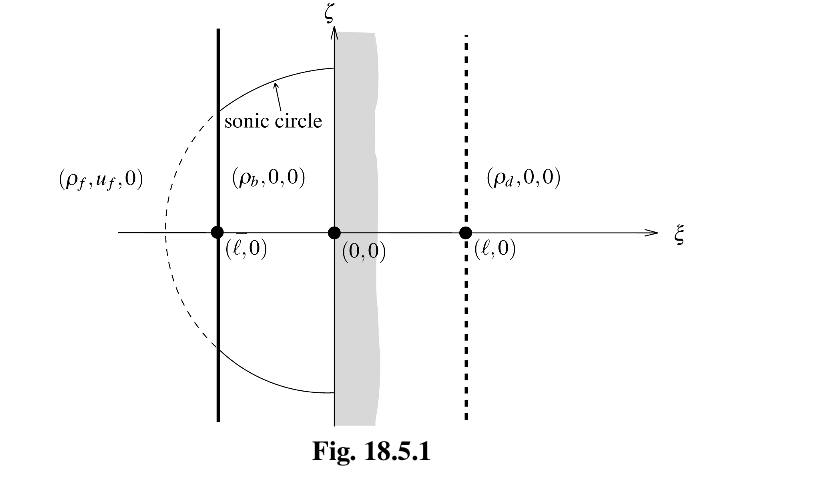
\includegraphics[width=0.7\textwidth]{ch18-fig05-01.png}
\caption{正反射：入射激波 $\xi=\ell$、反射激波 $\xi=\bar\ell$ 均平行于 $\zeta$ 轴；中间态 $(\rho_b,0,0)$ 的声速圆与反射激波相交。}
\label{figure:ch18-正反射}
\end{figure}

我们选取坐标使入射激波平行于 $y$ 轴，并沿 $x$ 轴正向运动。刚性壁由直线 $y=x\tan\omega$ 表示，其中 $\omega\in(0,\frac{\pi}{2}]$。入射激波连接左侧状态 $(\rho_f,u_f,0)$ 与右侧状态 $(\rho_d,0,0)$，在 $t=0$ 时位于 $y$ 轴上。由于几何与数据的伸缩不变性，流动是自相似的，如\cref{section:ch18-自相似无旋等熵气流}所说明，即 $\rho,u,v$ 与伪势 $\chi$ 是两个变量 $\xi=x/t$、$\zeta=y/t$ 的函数。

先考察正反射的最简单情形，即 $\omega=\pi/2$。若无壁面，入射激波本会沿 $x$ 方向推进，并在 $t=1$ 时占据坐标线 $x=\ell$，其中 $\ell>0$。于是在 $\xi$-$\zeta$ 平面中，入射激波表现为定常直线 $\xi=\ell$。

借助跳跃条件\eqref{align:ch18-18314}与\eqref{align:ch18-18315}，它们在此退化为
\begin{align}
\ell(\rho_f-\rho_d)=\rho_fu_f,
\label{align:ch18-1851}
\end{align}
\begin{align}
\ell u_f=\rho_f^{\gamma-1}-\rho_d^{\gamma-1}+\frac12 u_f^2,
\label{align:ch18-1852}
\end{align}
可一起确定 $\ell$ 以及 $\rho_f,u_f$ 与 $u_d$ 之间所需关系。联立得
\begin{align}
\frac{(\rho_f^{\gamma-1}-\rho_d^{\gamma-1})(\rho_f-\rho_d)}{\rho_f+\rho_d}
=\frac12 u_f^2,
\label{align:ch18-1853}
\end{align}
由此唯一确定 $\rho_d<\rho_f$。再由\eqref{align:ch18-1851}以 $u_f$ 与 $\rho_f$ 表出 $\ell$。

由于壁面，$t=0$ 时入射激波将被另一道激波反射，后者也平行于 $y$ 轴，但沿 $x$ 轴负向运动。在 $\xi$-$\zeta$ 平面中，该激波表现为坐标线 $\xi=\bar\ell$，其中 $\bar\ell<0$。反射激波的前面状态为 $(\rho_f,u_f,0)$，后状态为 $(\rho_b,u_b,v_b)$。壁面上法向速度分量必为零，故 $u_b=0$。又切向速度分量跨过激波必连续，故 $v_b=0$。剩余参数 $\rho_b$ 与 $\bar\ell$ 借助跳跃条件\eqref{align:ch18-18315}与\eqref{align:ch18-18316}确定，它们现在取形式
\begin{align}
\bar\ell(\rho_f-\rho_b)=\rho_fu_f,
\label{align:ch18-1854}
\end{align}
\begin{align}
\bar\ell u_f=\rho_f^{\gamma-1}-\rho_b^{\gamma-1}+\frac12 u_f^2.
\label{align:ch18-1855}
\end{align}
联立\eqref{align:ch18-1854}与\eqref{align:ch18-1855}得
\begin{align}
\frac{(\rho_f^{\gamma-1}-\rho_b^{\gamma-1})(\rho_f-\rho_b)}{\rho_f+\rho_b}
=\frac12 u_f^2,
\label{align:ch18-1856}
\end{align}
它唯一确定 $\rho_b>\rho_f$。再由\eqref{align:ch18-1854}算出 $\bar\ell$。一个简单估计表明，对任意 $\gamma>1$，
\begin{align}
|\bar\ell|<c(\rho_b)=\sqrt{\gamma-1}\,\rho_b^{\frac{\gamma-1}{2}},
\label{align:ch18-1857}
\end{align}
它意味着激波与状态 $(\rho_b,0,0)$ 的声速圆相交，如图\cref{figure:ch18-正反射}所示。因而反射激波一部分超声速、一部分跨声速。

现在转向斜反射情形，即 $\omega<\pi/2$。在 $\xi$-$\zeta$ 平面上，入射激波在点 $(\ell,\ell\tan\omega)$ 与壁面接触，并落在坐标线 $\xi=\ell$ 上。完全同上，借助跳跃条件\eqref{align:ch18-1851}与\eqref{align:ch18-1852}，再过渡到\eqref{align:ch18-1853}，可确定 $\ell$ 以及 $\rho_f,u_f$ 与 $\rho_d$ 之间所需关系。

\begin{figure}[ht]
\centering
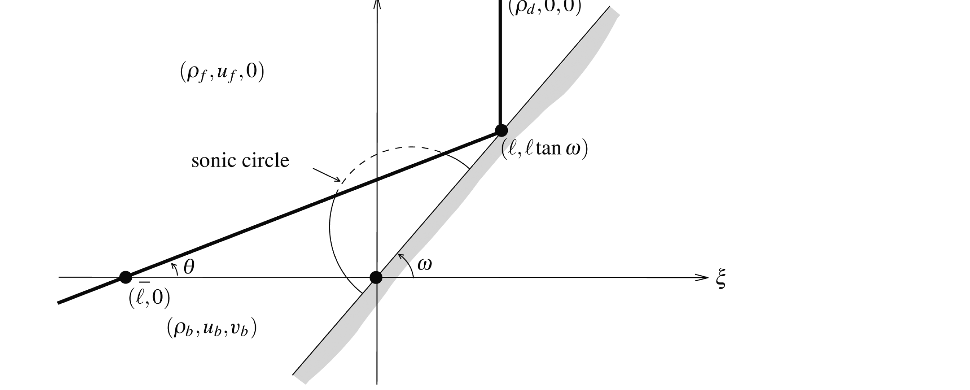
\includegraphics[width=0.85\textwidth]{ch18-fig05-02.png}
\caption{斜正规反射：入射激波在 $(\ell,\ell\tan\omega)$ 与壁面相遇，反射激波斜率为 $\tan\theta$，连接 $(\rho_f,u_f,0)$ 与 $(\rho_b,u_b,v_b)$。}
\label{figure:ch18-斜反射}
\end{figure}

要发生正规反射，必须配一道从点 $(\ell,\ell\tan\omega)$ 发出、斜率设为 $\tan\theta$、$\theta<\omega$、连接前面状态 $(\rho_f,u_f,0)$ 与某后状态 $(\rho_b,u_b,v_b)$（$\rho_b>\rho_f$）的激波；见图\cref{figure:ch18-斜反射}。速度场 $(u_b,v_b)$ 所需满足的条件是
\begin{align}
v_b-u_b\tan\omega=0,
\label{align:ch18-1858}
\end{align}
使壁面上法向速度为零；以及
\begin{align}
u_b+v_b\tan\theta=u_f,
\label{align:ch18-1859}
\end{align}
以满足速度切向分量跨过激波连续的要求。上述两方程给出
\begin{align}
u_b=\frac{1}{1+\tan\omega\tan\theta}u_f,\qquad
v_b=\frac{\tan\omega}{1+\tan\omega\tan\theta}u_f.
\label{align:ch18-18510}
\end{align}
为确定剩余参数 $\rho_b$ 与 $\theta$，借助跳跃条件\eqref{align:ch18-18315}与\eqref{align:ch18-18316}，它们在此退化为
\begin{align}
\ell(\rho_b-\rho_f)=\frac{\tan\theta}{\tan\omega-\tan\theta}\rho_fu_f
+\frac{v_b-u_b\tan\theta}{\tan\omega-\tan\theta}\rho_b,
\label{align:ch18-18511}
\end{align}
\begin{align}
\frac12 u_b^2+\frac12 v_b^2-\ell(u_b+v_b\tan\omega)
=\rho_f^{\gamma-1}-\rho_b^{\gamma-1}+\frac12 u_f^2-\ell u_f.
\label{align:ch18-18512}
\end{align}
将\eqref{align:ch18-18510}中的 $u_b$、$v_b$ 代入\eqref{align:ch18-18511}、\eqref{align:ch18-18512}，再在所得两方程之间消去 $\rho_b$，得到关于未知斜率 $\tan\theta$ 的单个方程。由\cref{section:ch18-定常平面等熵气流}中的讨论可知，只要 $\omega_d\leqslant\omega<\pi/2$，其中 $\omega_d\in(0,\frac12\pi)$ 称为脱体角，该方程就有满足 $\tan\theta<\tan\omega$ 的解。然后借助\eqref{align:ch18-18510}与\eqref{align:ch18-18511}可定出两个不同状态 $(\rho_b,u_b,v_b)$，一个由强激波连接到 $(\rho_f,u_f,0)$，另一个由弱激波连接。如\cref{section:ch18-超声速绕凸角}中所指出，强激波在实验中观测不到，故此处只保留弱激波。事实上，当 $\omega\to\pi/2$ 时，弱激波生成的波型收敛到前面描述的正反射波型。

当 $\omega$ 接近 $\pi/2$ 时，所得波型如图\cref{figure:ch18-斜反射}所示。我们观察到：状态 $(\rho_b,u_b,v_b)$ 的声速圆（圆心在壁面上的点 $(u_b,v_b)$，半径 $c(\rho_b)$）与反射激波相交，故该激波一部分超声速、一部分跨声速。然而接触点 $(\ell,\ell\tan\omega)$ 位于声速圆之外，故碰撞是超声速的。只要 $\omega_s<\omega<\pi/2$，其中 $\omega_s\in(\omega_d,\frac12\pi)$ 称为声速角，这一波型就持续。当 $\omega\in(\omega_d,\omega_s)$ 时，$(\ell,\ell\tan\omega)$ 位于声速圆之内，故反射是跨声速的。

当 $\omega<\omega_d$ 时正规反射不可能。数值与实验证据表明：在这种条件下，反射点与壁面脱开，但仍与之相连，形成一道称为 Mach 杆的复杂波型。尽管对这一称为 Mach 反射的现象已有大量研究，严格而确定的解析理论仍付诸阙如。涡旋面在 Mach 杆结构中起重要作用，因而势流似乎不能为这种理论提供合适的框架。

\end{document}
